\renewcommand{\thechapter}{6}

\chapter{The evolution of BECs in disordered potentials}

In this chapter, we report the experimental study of the evolution of BECs in disordered potentials. In Sec.~(\ref{optical_design}), we present the optical design diagrams of both the speckle beam and the Raman beams which are used to generate spin-orbit coupling as discussed in Sec.~(\ref{soc}). And we discuss the reasons behind these designs. In Sec.~(\ref{speckle_pulsing}), we show the experimental results of the evolution of BECs under the pulses of speckle potentials, both in the short term and in the long term. Based on our analytical study and numerical simulations, we show the results of characterizing the PSD of the speckle potentials by using the short-term speckle pulses data and measuring the average speckle potential by using the long-term speckle pulses data. In Sec.~(\ref{transport}), we measure the deceleration of spinless BECs in the speckle potentials and compare them with our simulation results shown in Ch. (\ref{chpt 5}).
\section{Optical design}

\subsection{Speckle beam design}\label{speckle_design}

\begin{figure*}
    \centering
    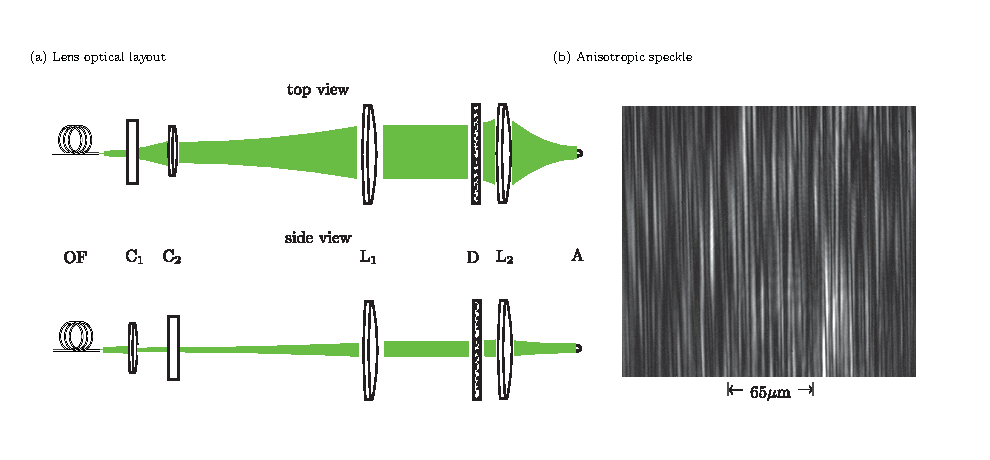
\includegraphics{Chapter6_secs/speckle_design.pdf}
    \caption{Optical design. (a). The design of optics viewed in two directions. OF denotes optical fiber. Lenses $C_1$ and $C_2$ are cylindrical lenses: $C_1$ focuses the beam in the vertical direction; and $C_2$ focuses the beam in the horizontal direction. $L_1$ is a spherical lens that collimates the beam. D is the optical diffuser that imprints random phase on the beam. $L_2$ is an aspherical lens that focuses the beam to the atoms labelled with A. (b) Experimental image of optical speckle with anisotropic correlation length.}
    \label{fig:design}
\end{figure*}

In practice, the speckle beam must satisfy two requirements.
The first is anisotropic field-field correlation length: small along $\ex$ and large along $\ey$ and $\ez$ so that high-momentum scattering occurs predominantly along $\ex$. 
The second is that the beam width along $\ex$ should uniformly illuminate the elongated atomic ensemble (with expected diameter of about $50\ \mu{\rm m}$).
To observe the effect of SOC-suppressed transport, the speckle potential must couple energy matched states across the SOC gap, shown by the dashed line in Fig.~\ref{fig:Dispersion relations}(c). 
This implies PSD of speckle potential along $\ex$ satisfies $k_c\gtrsim 4\kr$, informing the selection of beam-size and lenses.
The requirement that the correlation length along $\ey$ be large implies that at the diffuser plate, the beam be much smaller along $\ey$ than along $\ex$.

To satisfy these joint requirements, we created the speckle beam shown in Fig.~\ref{fig:design}(a), that begins with a $532{\rm nm}$ laser beam emanating from an optical fiber. 
The beam out of an optical fiber travels through the cylindrical lens $C_1$ (focusing along $\ey$) before encountering a cylindrical lens $C_2$ (focusing along $\ex$) as shown in Fig.~\ref{fig:design}(a), given more rapid divergence along $\ex$ than $\ey$.
The beam is then collimated by $L_1$, a $f = 250\ {\rm mm}$ spherical lens, giving beam width of around $25\ {\rm mm}$ along $\ex$ and less than $500\ \mu{\rm  m}$ along $\ey$ (on the same scale the diffuser plate's correlation length). 

The beam then traverses the diffuser plate (Edmund Optics part number \#47-680, with divergence angle $\theta_d = 0.5^\circ$)  and is focused by $L_2$, a $f = 30\ {\rm mm}$ lens.
Figure~\ref{fig:design}(b) shows a test image of the speckle beam at the focal plane, its intensity correlation length is less than $0.5\ {\rm \mu m}$ along $\ex$ and about $10\ \mu{\rm  m}$ along $\ey$. 
The beam widths along both directions are about $250\ \mu{\rm m}$.


\subsection{Raman beams design}
We generate Raman coupling with $\lambda \approx {\rm 790nm}$ laser. The recoil vector of the laser is 
\begin{equation}
   k_{\rm r} = \frac{2\pi}{\lambda}.
\end{equation}
When two Raman beams intersect at an angle $\theta_R$ as shown in Fig.~(\ref{fig:raman_design}), the two photon recoil vector is
\begin{equation}
    \kr = k_{\rm r}\sin{\frac{\theta_R}{2}}.
\end{equation}
As shown in Fig.~(\ref{fig:Dispersion relations}c), the detuning between states $\ket{q+\kr,\uparrow}$ and $\ket{q-\kr,\downarrow}$ is
\begin{equation}
    \Delta(q) = \frac{2\hbar^2q\kr}{m} + \delta.
\end{equation}
$\delta$ here is the detuning between two Raman beams and $\Delta(q)$ increases with $\kr$. As described in Sec.~(\ref{soc}), one step in the process we prepare the SOC quasimomentum state $\ket{q_0,-}$ is adiabatic evolution. We achieve this by ramping up the Raman coupling strength from zero to $\Or$ on a time scale slow compared to $\hbar/\Delta(q_0,0)$. In experiment, we prefer to ramp up Raman coupling fast, limited by the lifetime of BEC, but still slow compare to $\hbar/\Delta(q_0,0)$. For this reason, we want to make $\kr$ as large as possible. In this design, it means large enough intersection angle $\theta_R$. On the other hand, we also want $\kr$ to be small enough that $k_c/\kr$ is large enough the speckle potential can couple more energy matching stats shown as the circles in Fig.~(\ref{fig:Dispersion relations}). Here $k_c$ is the cut off in the PSD of the speckle potential. In our experiment, the two Raman beams and the speckle beam are focused to the atoms by the same lens $L_1$, at the largest $\theta_R$, $k_c/\kr \approx 3$. 

For the above two reasons, there is a trade off between small and large $\theta_R$, we need to find out the best angle by experimentally test. So for the optical design, we need to be flexible in changing the angle. As shown in Fig.~(\ref{fig:raman_design}), we use a triangular prism to combine the two Raman beams and align them to be parallel. The triangular prism is put on a transnational stage which can move in the perpendicular direction of the two incident Raman beams. By moving the prism, the distance between the two Raman beams can be changed and the distance is map to the distance at lens $L_1$ which determines the angle $\theta_R$.

\begin{figure*}
    \centering
    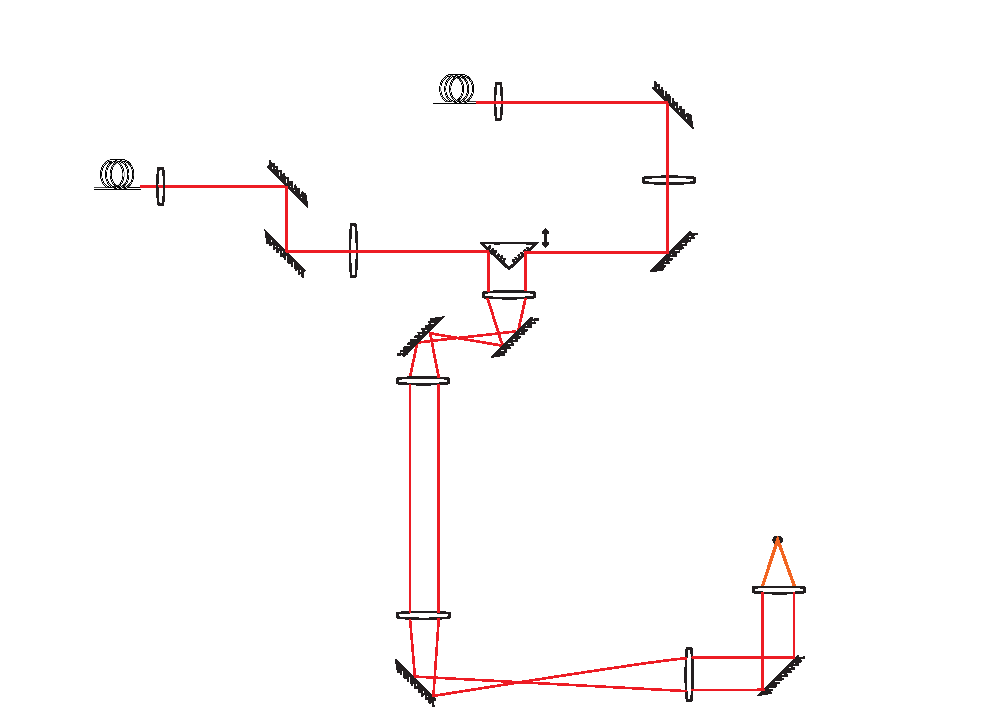
\includegraphics{Chapter6_secs/Raman_design.pdf}
    \caption{Raman beams design. The optical diagram of Raman beams. We use a triangular prism to align two Raman beams, the distance between two Raman beams at the prism is mapped to the distance at the lens $L_1$ by two relay imaging systems. The prism is put on a transnational stage which can move in the perpendicular direction of the two incident Raman beams. By moving the prism, the distance between the two Raman beams can be changed which determines the angle $\theta_R$.}
    \label{fig:raman_design}
\end{figure*}
\section{Evolution of spinless BEC under speckle pulsing}\label{speckle_pulsing}
In Ch.~(\ref{speckle_chapter}), we derived a Gaussian beam model of the speckle beam and calculated the field-field correlation function, the PSD, and the intensity distribution. In the experiments, the engineered speckle beam is focused at the atoms and it is hard to directly measure the average intensity of the speckle beam at the atoms. Direct measurements of the PSD and $k_c$ is even harder. In some experiments carried out previously that involved a speckle beam \cite{kondov2011three, billy2008direct}, the researchers set up an identical beam at the test bench and measure the average intensity and the PSD of the test speckle beam. The power and the PSD of the speckle beam in the experiments are assumed to be the same as those of the test beam, but no direct measurements were done to the best of our knowledge. Inspired by \cite{huckans2009quantum}, we designed and carried out an experiment that allowed us to measure the average intensity and the PSD of the speckle beam by using the evolution of spinless BECs under the speckle potentials.

\begin{figure*}
    \centering
    \includegraphics{Chapter6_secs/speckle_pulsing_images.pdf}
    \caption{Absorption images of atoms after the evolution under speckle potentials and TOF. The BECs are released from the dipole trap, the pulses of the speckle potentials are turned on immediately for a various amount of time, followed by TOF. The absorption images are stacked up horizontally according to the speckle pulse duration.}
    \label{fig:speckle_pulsing_imgs}
\end{figure*}

In \cite{huckans2009quantum}, the diffraction of a Bose-Einstein condensate from a one-dimensional optical lattice is studied. In very short time,
\begin{equation}
    T_{pulse} \ll t_{RN} = \frac{\hbar}{\sqrt{U_0E_L}} = \frac{T_{ho}}{\pi},
\end{equation}
the atoms are mainly scattered to the $\ket{\pm k_L}$ momentum states. Since in the Raman-Nath approximation, the atoms move by a very small distance, the kinetic energy term in the Hamiltonian is neglected. The atomic momentum changes from $\ket{k=0}$ to $\ket{\pm k_L}$, which corresponds to the nonzero components in the PSD of the lattice potential. This inspires us to measure the PSD of the speckle potential and the cutoff $k_c$ by using the short-term speckle beam pulses.

As the pulse duration increases beyond $t_{RN}$, the apparent edge of the momentum distribution is bounded by a maximum momentum $k_{max}$. The observed value of $k_{max}$ can be used to determine the lattice depth $U_0$,
\begin{equation}
    U_0 = \frac{\hbar^2k_{max}^2}{2M}
\end{equation}
Once the edge of the distribution reaches $k_{max}$, the distribution partially collapses to $\ket{k=0}$ at $T_{ho}/2$. The process approximately repeats itself every $T_{ho}/2$. The collapse and revival phenomena can be qualitatively explained in a classical picture. The atoms released from different positions in a harmonic trap become stationary every half of the period. The collapse and revival are not complete in \cite{huckans2009quantum}, at $T_{ho}/2$ there are always some higher momentum orders remain. The reason is that the lattice potential is not perfectly harmonic. 

In contrast to the lattice pulsing, in the speckle beam pulsing, the speckle potential contains a continuous spectrum of spatial frequency. It is completely anharmonic and no collapse and revival should be expected. For long speckle pulsing time, the momentum states should reach a stationary distribution. By Virial theorem, the kinetic energy of the atoms under this stationary distribution should be half of the average speckle potential. This inspired us to measure the average speckle potential by using the width of the momentum distribution for a long speckle pulsing time.

% \begin{figure*}
%     \centering
%     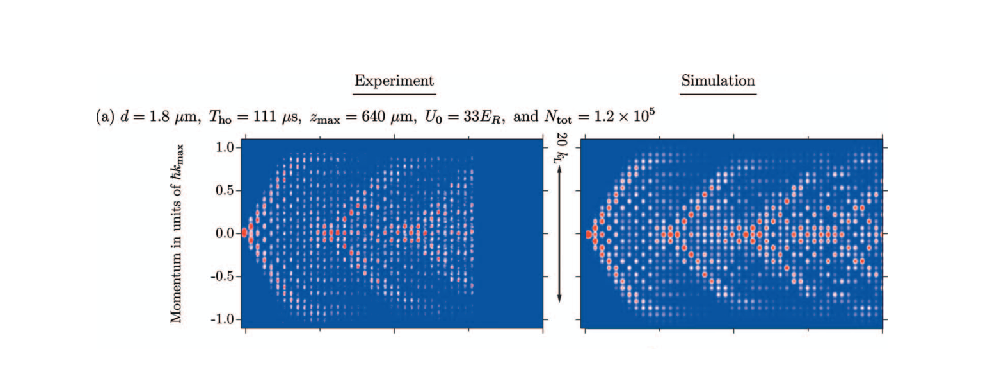
\includegraphics{Chapter6_secs/lattice_pulsing.pdf}
%     \caption{Fig.~1(a) of \cite{huckans2009quantum}. Concatenated absorption images of diffraction patterns, showing the evolving momentum distribution, compared with numerical GPE simulation results.}
%     \label{fig:lattice_pulsing}
% \end{figure*}

\subsection{Short term speckle pulsing}\label{short_pulse_sec}

To measure the PSD and the cutoff $k_c$ of the speckle potentials with short term speckle pulsing, we derive the evolution of the momentum states under two approximations. The first is the Raman-Nath approximation, atoms do not move far during the pulse.  The second is that the evolution time is short compared to $\hbar/V(x)$, so atoms do not acquire a phase comparable to $2\pi$.
Consider Hamiltonian
\begin{equation}
    \hat{H} = \frac{\hbar^2k^2}{2m} + V(x).
\end{equation}
The time evolution operator is
\begin{equation}
    \hat{U}(t) = \exp{-i\frac{\Delta t}{\hbar}\left[\frac{\hbar^2k^2}{2m}+V(x)\right]},
\end{equation}
Define $E_c$ as the energy associated with $k_c$, $\tau = \frac{\Delta t}{\hbar}E_c$, $\hat{k} = \frac{k}{k_c}$ and $S(x) = \frac{V(x)}{E_c}$
\begin{equation}
    \hat{U}(t) = \exp{-i\tau\left[\hat{k}^2+S(x)\right]}.
\end{equation}
Expand the operator to second order, 
\begin{equation}
    \hat{U}(t) = \exp{-i\tau\hat{k}^2/2}\exp{-i\tau S(x)}\exp{-i\tau\hat{k}^2/2}.
\end{equation}
We assume the initial state is $\ket{k=0}$, so the third term does not contribute. And we measure the distribution in $k$ space, so we can ignore the first term. The second term governs the short time evolution. To the lowest order, 
\begin{equation}
    \hat{U}(t)\ket{k=0} = \ket{k=0} - i\tau S(x) \ket{k=0}
\end{equation}
Expand $S(x)$ in $k$ space,
\begin{equation}
    S(x) = \sum_{k,k'}\Tilde{S}(k-k')\dyad{k}{k'}
\end{equation}
So
\begin{equation}
    \hat{U}(t)\ket{k=0} = \ket{k=0} - i\tau \sum_{\delta k}\Tilde{S}(\delta k)\ket{\delta k}
\end{equation}
The probability distribution of momentum states at time $\tau$ is
\begin{equation}\label{short_dist}
    P(k,\tau) = \tau^2 |\Tilde{S}(k)|^2 + \delta_{k,0}.
\end{equation}
It is proportional to the PSD of the speckle potential $|\Tilde{S}(k)|^2$ ignoring the central peak at $k=0$.

In the experiments, we put an iris right before the diffuser $D$ in \ref{fig:design}. By opening and closing the iris, we can control the size of the beam which determines $k_c$ of the speckle potential PSD in the focal plane. As the model we derived in Ch.~(\ref{speckle_chapter}) shows, the speckle beam size at the focal plane does not change with the beam size at the diffuser. The beam size at the focal plane is determined by the field-field correlation length at the diffuser. So the average speckle potential depth is proportional to the power of the beam which we can control when we change the size of the iris. 

We did the experiments for two iris sizes, $6.5\ {\rm mm}$ and $15\ {\rm mm}$, which correspond to $k_c=0.65k_r$ and $k_c=1.30k_r$, respectively. Here $k_r$ is defined with the largest recoil $k$ vector of atoms scattered by a $532\ {\rm nm}$ light beam focused by a one inch $f=30\ {\rm mm}$ lens. 
\begin{equation}
    k_r = \frac{2\pi}{532 {\rm nm}}\sin{\frac{\theta_{\rm R}}{2}}
\end{equation}
$\theta_{\rm R} \approx 45^\circ $ is shown in Fig.~(\ref{fig:raman_design}).
The average speckle potential match in both cases by controlling the power of the beam after the iris. 

We prepare BECs in a cross dipole trap, at $t=0$, we turn off the dipole trap and release the atoms for time-of-flight (TOF). Immediately after the dipole trap is turned off, we turn on the speckle beam and pulse for a short period of time, ranging from $20\ {\rm \mu s}$ to $250\ {\rm \mu s}$. After $18\ {\rm ms}$ TOF, we take absorption images of the atoms.

To compare with the experimental data, we simulate the process numerically. In the numerical simulation, we prepare the ground state of BECs in a dipole trap. At $t=0$, turn off the dipole trap and release the atoms. Immediately after, the speckle potential is turned on for a duration of $50\ {\rm \mu s}$ or $100\ {\rm \mu s}$, followed by free evolution for up to $20\ {\rm ms}$. We keep track of the momentum distribution of the atoms during the evolution. 

\begin{figure*}
    \centering
    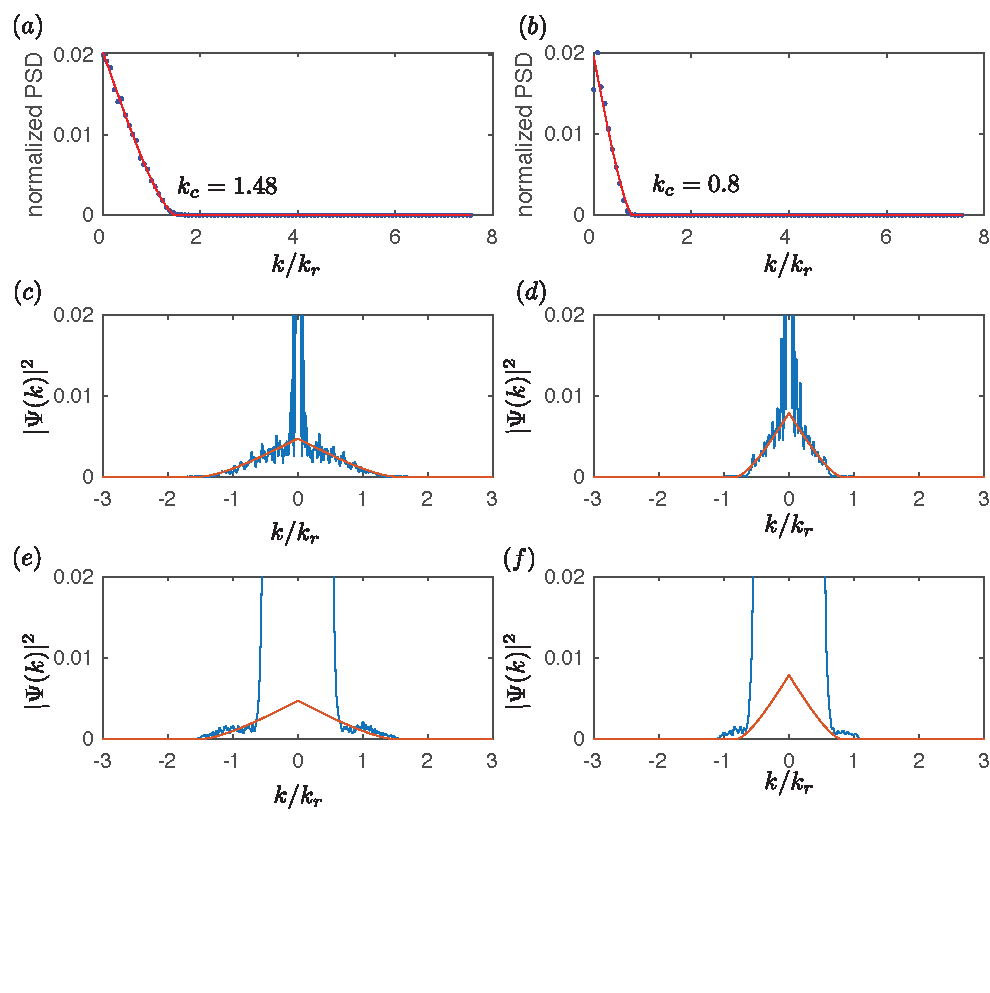
\includegraphics{Chapter6_secs/speckle_pulsing_simu.pdf}
    \caption{Simulation of short-term speckle pulsing. The left panel is for speckle potential with $k_c = 1.48k_r$, and the right panel for $k_c = 0.8k_r$. (a) and (b) verify the $k_c$ of both speckle potentials by plotting their PSD. (c) and (d) are the momentum distribution of atoms after released from the dipole trap and evolve under speckle pulses for $50\ {\rm \mu s}$. The red curves are proportional to the corresponding PSD of the speckle potential. The momentum distribution is an average of 20 speckle realizations. (e) and (f) are the momentum distribution of atoms after released from the dipole trap and evolve under speckle pulses for $50\ {\rm \mu s}$ followed by a $20\ {\rm ms}$ free expansion. The results are averaged over 20 speckle realizations. }
    \label{fig:speckle_pulsing_simu}
\end{figure*}

As Fig.~(\ref{fig:speckle_pulsing_simu}) shows, the simulation is done under two kinds of speckle potentials with different $k_c$ to compare with the experimental data. The left panel of Fig.~(\ref{fig:speckle_pulsing_simu}) is for the speckle potential with $k_c = 1.48k_r$ and the right panel for the speckle potential with $k_c = 0.80k_r$. Fig.~\ref{fig:speckle_pulsing_simu}(c) and Fig.~\ref{fig:speckle_pulsing_simu}(d) show the momentum distribution of atoms immediately after a $50\ {\rm \mu s}$ speckle pulsing, the results are averaged over 20 speckle realizations. The red curves are proportional to the PSD of the two kinds of speckle potentials, respectively. From Fig.~\ref{fig:speckle_pulsing_simu}(c) and Fig.~\ref{fig:speckle_pulsing_simu}(d) we can see the tail of the momentum distribution of atoms after short-term speckle pulsing matches with the PSD of the speckle potentials. The results agree with the analytical calculation of the momentum distribution in Eq.~(\ref{short_dist}), which predicts the momentum distribution to be a central $\delta$ function plus a tail that is proportional to the PSD of the speckle potentials. 

Fig.~\ref{fig:speckle_pulsing_simu}(e) and Fig.~\ref{fig:speckle_pulsing_simu}(f) show the momentum distribution of atoms after a $50\ {\rm \mu s}$ speckle pulse and a $20\ {\rm ms}$ time-of-flight (TOF). During the TOF, the mean-field expansion of the atoms broadens the momentum distribution. Both the central peak and the tail of the momentum distribution become broader after the TOF. In Fig.~\ref{fig:speckle_pulsing_simu}(f), for the speckle potential of smaller $k_c$, the tail of the momentum distribution is broadened more significantly. The broadened momentum distribution after TOF makes it harder to distinguish the speckle potentials with the tail of the momentum distribution.

\begin{figure*}
    \centering
    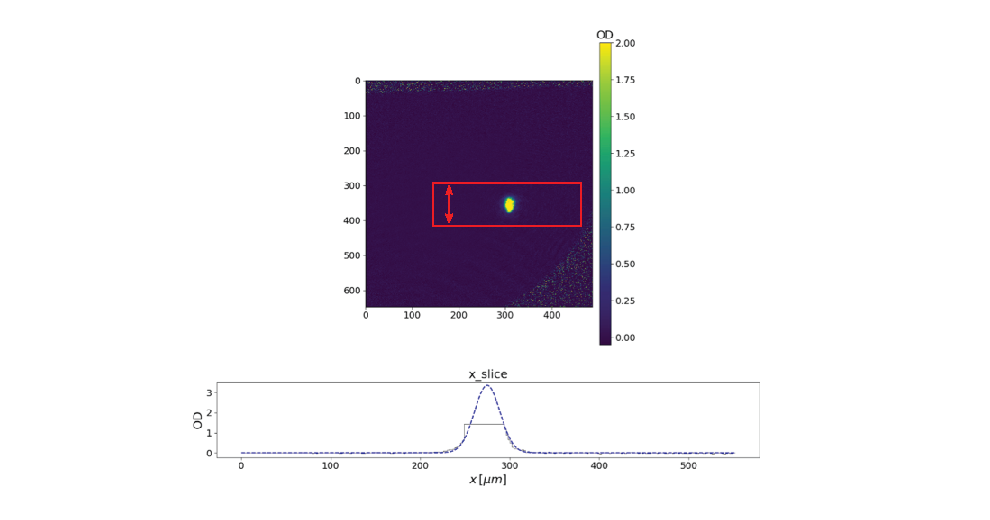
\includegraphics{Chapter6_secs/colOD.pdf}
    \caption{A sample of absorption images of atoms and analysis. The red square is a selected region of interest and the red arrow indicates the direction we take average. The masked and averaged spatial distribution of atoms (black curve) and a fitted Gaussian curve (blue dashed) are plotted below.}
    \label{fig:colOD}
\end{figure*}

\begin{figure*}
    \centering
    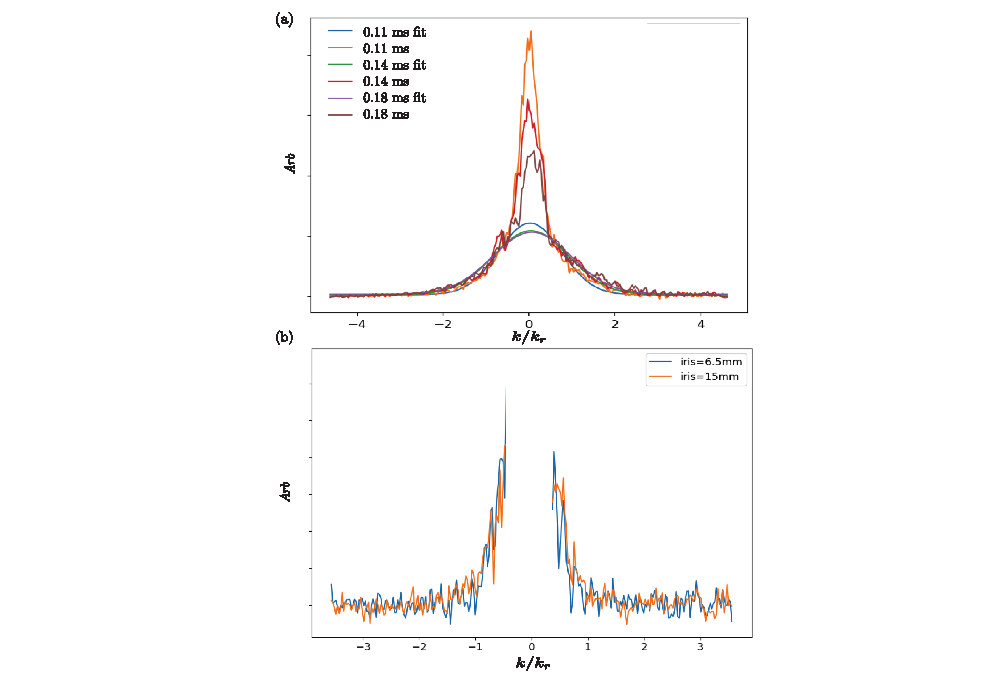
\includegraphics{Chapter6_secs/short_pulse.pdf}
    \caption{Momentum distribution after short-term speckle pulses and $18\ {\rm mm}$ TOF. (a). A few samples of momentum distribution of atoms without mask, along with fitted Gaussian curves to the masked momentum distribution. (b). The tails of the momentum distribution after short-term pulses of speckle potential with different PSD. The PSD of the speckle potentials are controlled by the iris sizes and the results are averaged for speckle pulsing time ranging from $80\ {\rm \mu s}$ to $150\ {\rm \mu s}$.}
    \label{fig:short_pulse}
\end{figure*}


Fig.~\ref{fig:colOD} and Fig.~\ref{fig:short_pulse} show the analysis results of the absorption images after TOF for two kinds of speckle potentials generated with different iris sizes. During TOF, the momentum distribution of atoms is mapped to their spatial distribution. From the absorption images, we can compute the momentum distribution from the spatial profile of the atoms. In the analysis, from the absorption images of atoms after TOF shown in Fig.~\ref{fig:colOD}, we select a region of interest around the center of the atoms indicated by the red square. And compute the average spatial distribution of atoms along the horizontal direction (red arrow). The central peak of this average spatial distribution is masked to show the detail of the tails. Fig.~\ref{fig:colOD} shows an example of the masked averaged spatial distribution along $x$ direction (black curve) and a Gaussian fit (blue dashed curve). The resultant tails of the spatial distribution are averaged over short-term speckle pulsing duration ranging from $80\ {\rm \mu s}$ to $150\ {\rm \mu s}$. The tails of the spatial distribution are then converted to that of the momentum distribution in a unit of $k_r$. 


Fig.~\ref{fig:short_pulse}(a) shows a few samples of the averaged momentum distribution along $x$ direction without a mask for short-term speckle pulsing, along with fitted Gaussian curves to the masked momentum distribution. From Fig.~\ref{fig:short_pulse}(a) we can see it is necessary to mask the central peak of the momentum distribution in order to analyze the width of the tails. Fig.~\ref{fig:short_pulse}(b) is the momentum distribution of atoms after short-term pulses of speckle potentials with different PSD, averaged over pulsing duration ranging from $80\ {\rm \mu s}$ to $150\ {\rm \mu s}$. From Fig.~\ref{fig:short_pulse}(b), it is hard to tell the difference between the two curves for two reasons. First, in the absorption images, the signal-noise-ratio at the tails of the density profile is low. Just by taking the average, it is hard to reduce the noise and see the clear tails as in the numerical simulation in Fig.~\ref{fig:speckle_pulsing_simu}. Second, as the simulation results show in Fig.~\ref{fig:speckle_pulsing_simu}(e) and Fig.~\ref{fig:speckle_pulsing_simu}(f), during TOF, the mean-field expansion broadens the momentum distribution more significantly for speckle pulsing with smaller $k_c$. So the width of the tails of the momentum distribution for the pulsing of two kinds of speckle potentials is closer to each other after TOF than before. For the two reasons, we conclude we can not quantitatively measure the $k_c$ of the speckle potential by using the absorption images after short-term speckle pulsing and TOF.



\subsection{Long term speckle pulsing}\label{long_pulse}

In the experiments, it is important to know the average speckle potential at the atoms. But unfortunately, it is hard to measure the power of the speckle beam directly at the atoms and infer the average speckle potential. Because in the experiments, we can not put a power meter anywhere we want to measure the power of the beam. And besides, it is the intensity that matters, and we don't have perfect knowledge of the beam size at the atoms. After the closest point to the vacuum glass cell where we can use a power meter to measure the power, the beam goes through lenses, reflected by mirrors, glass cell or even dichroic mirrors. The power of the beam decreases at each of the optical element. To the best of our knowledge, for the previous experiments using speckle beams, the average speckle potential was not measured directly. It could be inferred by calculating the power given the power loss at each optical element. Or the power could be measured for an identical speckle beam set up on the test bench and it is assumed the power at the atoms is the same as the power of the test speckle beam in the focal plane. 

Inspired by \cite{huckans2009quantum}, we obtained the mean potential depth by making the atoms evolve under the speckle beam pulses. Compared with \cite{huckans2009quantum}, for $t \gg t_{RN}$, we do not expect to see the collapse and revive phenomenon due to the anharmonicity of the speckle potential. Instead, at long speckle pulsing time, the momentum distribution should reach equilibrium and by virial theorem, the average stationary kinetic energy is half of the average total energy which is the initial average speckle potential. 

To confirm our understanding, we did numerical simulations of the long-term speckle pulsing. Fig.~\ref{fig:speckle_pulsing} shows the simulation and experimental results of the speckle pulsing for the pulsing duration up to $2\ {\rm ms}$. In the simulation, we release the BECs from the dipole trap and immediately turn on the speckle potential. The atoms evolve under the speckle potential and we keep track of the width of the momentum distribution. We did the simulation for different average speckle potential depth ranging from $0\ {\rm Hz}$ to $1600\ {\rm Hz}$, with a $200\ {\rm Hz}$ spacing. The results are shown as the nine curves, each one is averaged over 20 speckle realizations. When the average speckle potential is zero, the width of the momentum distribution increases driven by the mean-field expansion. From the simulation results shown in Fig.~\ref{fig:speckle_pulsing}(a), the width of the momentum distribution increases rapidly after the speckle potential is turned on and becomes stationary after around $0.25\ {\mu s}$. The stationary width increases with the average speckle potential depth. Fig.~\ref{fig:speckle_pulsing}(b) shows the experimental results. In the experiment, we release the atoms from the dipole trap, pulse the speckle potential for up to $2\ {\rm mm}$ followed by TOF. The total time for the speckle pulsing and the TOF is $18\ {\rm ms}$, a constant for different pulsing duration. We take the absorption images after TOF and fit a Gaussian function to the density profile of the atoms. Fig.~\ref{fig:speckle_pulsing}(b) shows the width of the fitted Gaussian function vs the duration of the speckle pulses. The Gaussian width increases with the pulsing duration in short term and becomes stationary after around $0.25\ {\rm ms}$, which is consistent with the simulation results. 

\begin{figure*}
    \centering
    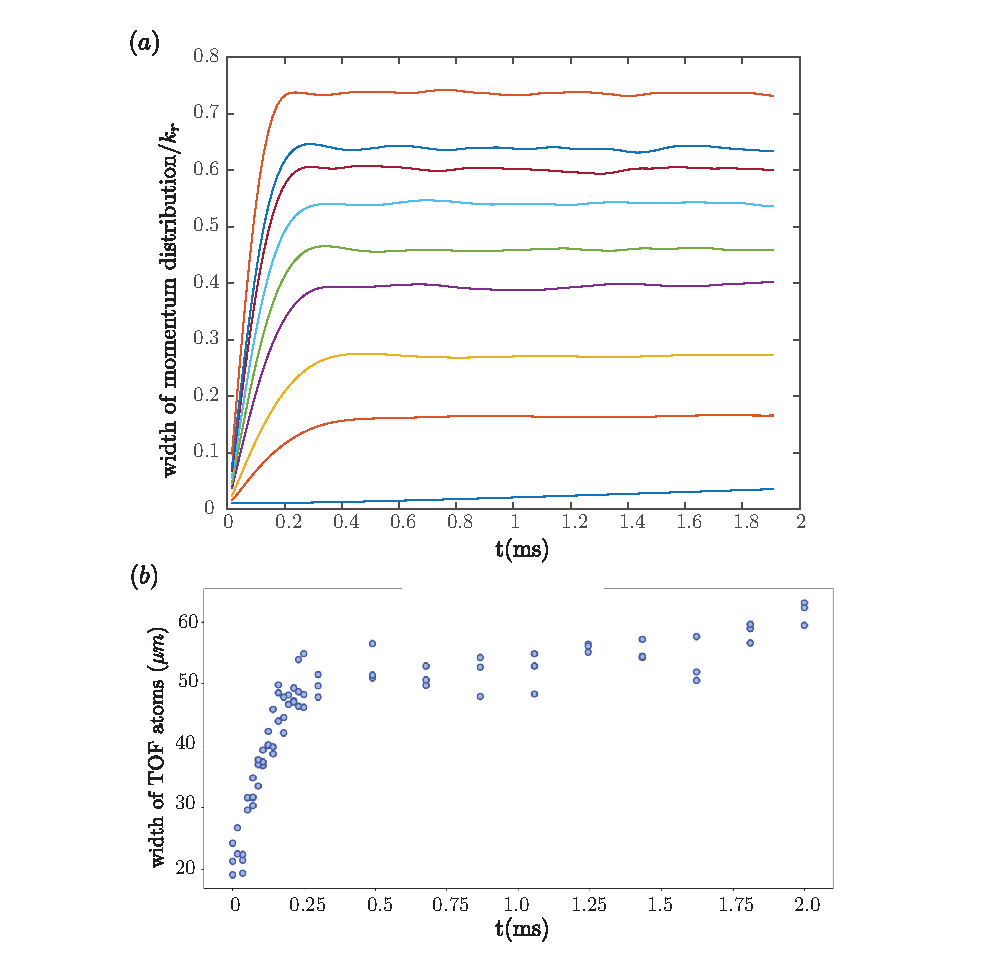
\includegraphics{Chapter6_secs/speckle_pulsing_width.pdf}
    \caption{The simulation and the experiments of the speckle beam pulsing. (a). The width of the momentum distribution of atoms evolving under the speckle potentials of different potential depth ranging from $0$ to $1600\ {\rm Hz}$.  (b). The Gaussian width of atoms in the absorption images after TOF for different speckle pulsing duration.}
    \label{fig:speckle_pulsing}
\end{figure*}

To infer the average speckle potential from the width of the momentum distribution after long-term speckle pulsing, we compute the average kinetic energy using the fitted Gaussian width of the density profile of atoms after TOF.
\begin{equation}
    \langle \hat{K} \rangle = \frac{1}{2} m \left(\frac{\sigma}{\tau}\right)^2
\end{equation}
Here $\tau$ is the time for TOF. The average speckle potential is equal to the average total energy, which by virial theorem is twice the average kinetic energy. In Fig.~\ref{fig:avg_speckle_poten}(b), the computed total energy is plotted against a photo diode (PD) reading. In our experiments, we use a pick-off mirror to reflect a fixed percentage of the power of the speckle beam to a PD and the reading of the PD in Volt is proportional to the power of the beam at the atoms. We fit a line crossing the origin to the data, by reading the PD we have an estimate of the average speckle potential at the atoms. 

To compare with the experimental results, we also did numerical simulations. In the simulations, we release the atoms from the dipole trap at $t=0$ and pulse the speckle potential for $1\ {\rm ms}$ followed by a $20\ {\rm ms}$ free evolution. The simulations are done with two kinds of speckle potentials, $k_c=0.80k_r$ and $k_c=1.48k_r$, respectively. For each kind of the speckle potential, the average potential depth ranges from $0\ {\rm Hz}$ to $1600\ {\rm Hz}$ with a $200\ {\rm Hz}$ spacing. We compute the momentum distribution and the average kinetic energy at the end of the free evolution. The average total energy is twice the average kinetic energy deducted by the mean-field energy computed from the average kinetic energy in the no-pulsing case. And the resultant average total energy is plotted against the known average potential depth. In agreement with our prediction, the curves are close to the diagonal line (dashed) for both kinds of speckle potentials.


\begin{figure*}
    \centering
    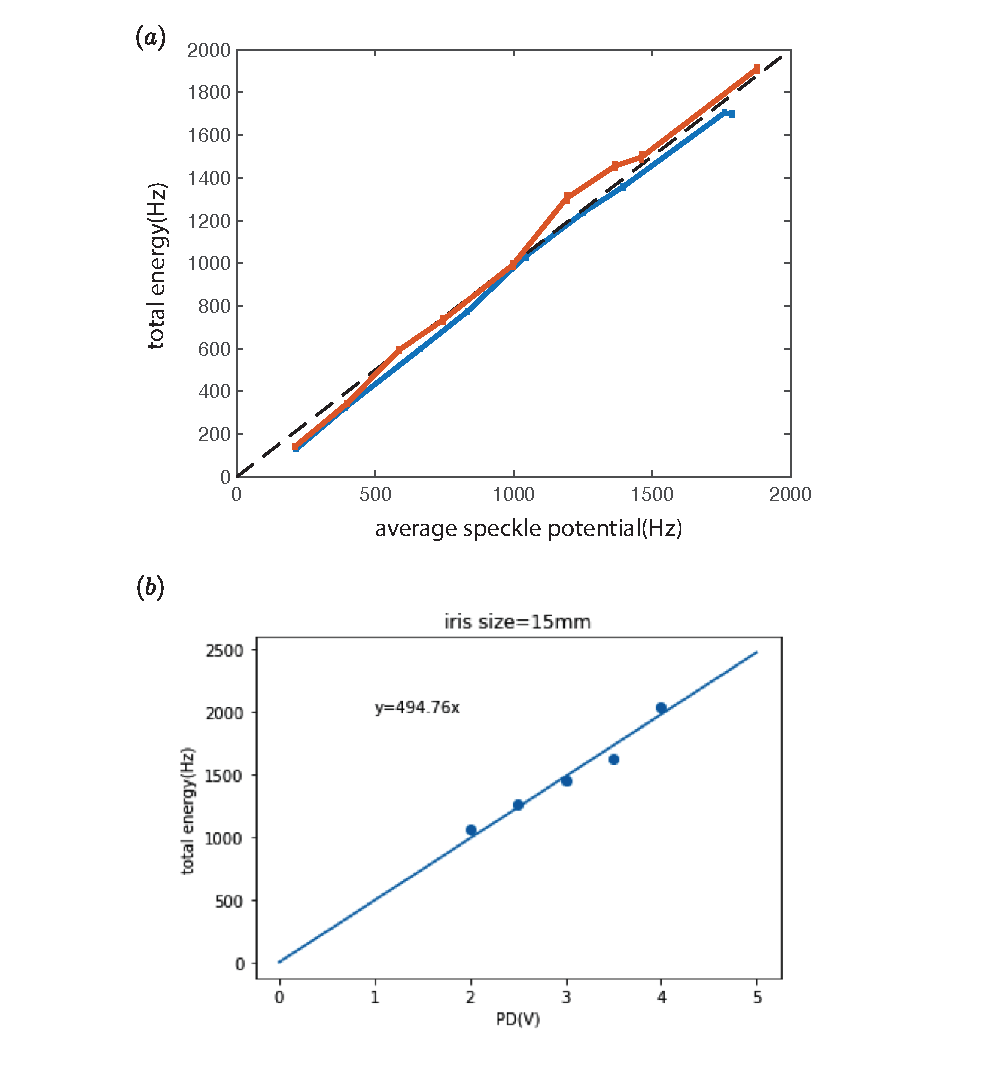
\includegraphics{Chapter6_secs/average_speckle_potential.pdf}
    \caption{Calibration of the average speckle potential depth. (a). In the numerical simulation, the average total energy inferred from the momentum distribution after $20\ {\rm ms}$ free evolution is plotted against the known average speckle potential depth. The red curve and the blue curve are for the speckle potentials with $k_c = 0.80k_r$ and $k_c=1.48k_r$, respectively. The dashed line is diagonal. (b). In the experiment, the average total energy computed from long-term speckle pulsing data is plotted against the PD reading.}
    \label{fig:avg_speckle_poten}
\end{figure*}




\section{Transport of spinless BECs in speckle potentials}\label{transport}

In Ch.~(\ref{chpt 5}), we study the transport of spinless BECs under speckle potentials. As Fig.~(\ref{fig:single}) shows, a BEC with a chemical potential $\sim 300\ {\rm Hz}$ travels through speckle potentials with average potential depth $\sim 200\ {\rm Hz}$, could be scattered by the speckle potential and decelerate. The deceleration of a BEC depends on its initial velocity, the speckle potential depth, and the cutoff $k_c$ in the speckle potential PSD. As Fig.~\ref{fig:single}(d) shows, after evolving under the speckle potentials for $16\ {\rm mm}$, the BECs with small initial velocity has more significant deceleration. For BECs with large initial velocity, $k_0>k_c/2$, the deceleration is minimal during the $16\ {\rm mm}$.

In the experiments, we study how BECs with different velocities decelerate. As discussed in Ch.~(\ref{speckle_chapter}), we can make speckle potentials that have the same PSD as the ones we use in our numerical simulations. And as discussed in Sec.~(\ref{speckle_pulsing}), the average speckle potential depth can be inferred from a PD reading. So an ideal experimental sequence is to have the BEC travel with constant velocity under well-calibrated speckle potential, and the final velocity would be measured by using $insitu$ or TOF absorption images. To that end, the first challenge we are faced with is that how to make a BEC travel with a constant velocity for an extensive amount of time ($16\ {\rm mm}$ in the simulation). We make BECs by doing evaporative cooling in a cross dipole trap as discussed in Sec.~(\ref{dipole trap}), so our first choice is to make BECs travel in the cross dipole trap. As Eq.~(\ref{dipole_poten}) suggests, dipole potential is proportional to the intensity of the dipole beam. 

In our case, as discussed in \ref{speckle_design}, we image atoms in $z$ direction and measure the motion of atoms in $x$ direction. The dipole potential in $x$ direction is a combination of the dipole potential from $z$ dipole beam and $x$ dipole beam. The width of the dipole potential from $x$ dipole beam is the Rayleigh range, which in our case is $\sim 1.3\ {\rm mm}$. Based on our design, the velocity of atoms corresponds to the recoil $k$ vector $k_r$ is $3.3\ {\rm \mu m/ms}$. We expect the atoms to move less than $50\ {\rm \mu m}$ during the experiment, so the dipole potential from x dipole beam can be ignored.

In $x$ direction, the dipole potential from the $z$ dipole beam is
\begin{equation}
    V_{dip}(x) = -V_0\exp{-\frac{2x^2}{w^2}}.
\end{equation}
where $w$ is the width of the beam at the atoms. Expand the potential at $x=0$ to second order,
\begin{equation}
    V_{dip}(x) \approx -V_0 + \frac{2V_0}{w^2}x^2,
\end{equation}
has a quadratic form. Around the center of the trap, the dipole potential can be approximated by a harmonic potential with frequency $\sqrt{\frac{4V_0}{w^2}}$.

In the ideal case, the atoms would move at a constant velocity in the dipole trap, meaning the frequency $\sqrt{\frac{4V_0}{w^2}}$ is zero and the $z$ dipole beam is completely turned off. More realistically, if the velocity of the atoms change by less than 5\% at the center of the trap in $15\ {\rm ms}$, the period of the harmonic oscillation needs to be more than $300\ {\rm ms}$. So the trapping frequency is around $3\ {\rm Hz}$. 

The $x$ dipole beam and the $z$ dipole beam in our experiments are the first order and zeroth-order beams from an AOM, the total power of the two beams are conserved. We optimized the ratio of the power of the two beams to maximize the phase space density of the BECs after the dipole evaporation stage. In the optimized case, the measured trapping frequency in $x$ direction is $21\ {\rm Hz}$. In order to decrease the $x$ trapping frequency, we need to allocate more power in the $x$ dipole beam and less in the $z$ dipole beam. But in the process of decreasing the $x$ trapping frequency, a few problems occurred. 

Fig.~\ref{fig:lower trapping freq} shows the BEC with $x$ trapping frequency of $21\ {\rm Hz}$ compared with the BEC with $x$ trapping frequency of $5.8\ {\rm Hz}$. Compared with the BEC in Fig.~\ref{fig:lower trapping freq}(a), the BEC in Fig.~\ref{fig:lower trapping freq}(b) is stretched in the $x$ direction due to small trapping frequency. The signal is much weaker and the large length in $x$ direction makes it hard to accurately detect the center of the atoms and the center-of-mass motion.

\begin{figure*}
    \centering
    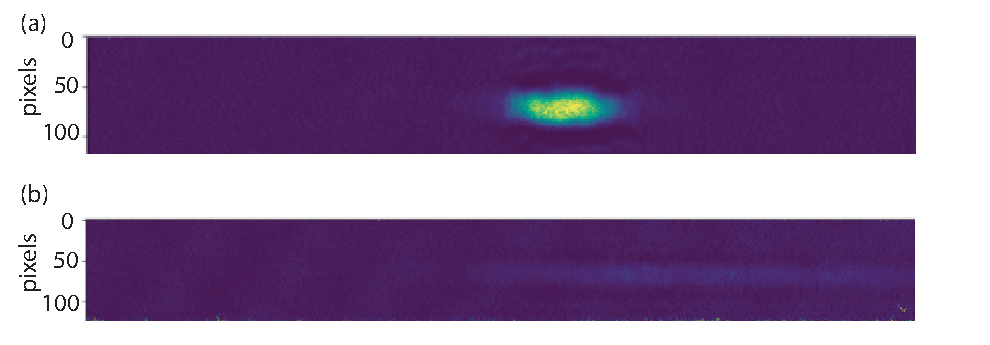
\includegraphics{Chapter6_secs/decrease_trap_freq.pdf}
    \caption{$insitu$ absorption images of BECs with different dipole parameters. (a) A BEC with $x$ trapping frequency of $21\ {\rm Hz}$. (b) A BEC with $x$ trapping frequency of $5.8\ {\rm Hz}$}
    \label{fig:lower trapping freq}
\end{figure*}

Alternatively, we can keep the current dipole trap configuration and decrease the time that BECs travel under speckle potentials. We hope to find the duration of the speckle potential pulses that is as short as possible, but its deceleration effect on the BECs is still significant for speckle potential weak enough not to cause trapping effect. 

In Fig.~\ref{fig:deceleration_in_dip_osc}, the blue dots show the oscillation of a BEC in $x$ direction in a dipole trap with $x$ trapping frequency $21\ {\rm Hz}$. The center of the atoms is measured from $insitu$ images of atoms. At the center of the dipole trap, the atoms are at the maximum velocity $v_0$, $mv_0/\hbar = 1.8k_r$. The first time the atoms reach maximum velocity is at $21\ {\rm ms}$. We make the atoms do the same dipole oscillation as the blue dots show, at $21\ {\rm ms}$, we turn on the speckle potential and hold for $1\ {\rm ms}$. After $1\ {\rm ms}$, the speckle potential is turned off and we track the center-of-mass motion of the atoms in $x$ direction in the dipole trap. The center-of-mass motion of atoms after the speckle pulse is shown as the orange dots in Fig.~\ref{fig:deceleration_in_dip_osc}. 

\begin{figure*}
    \centering
    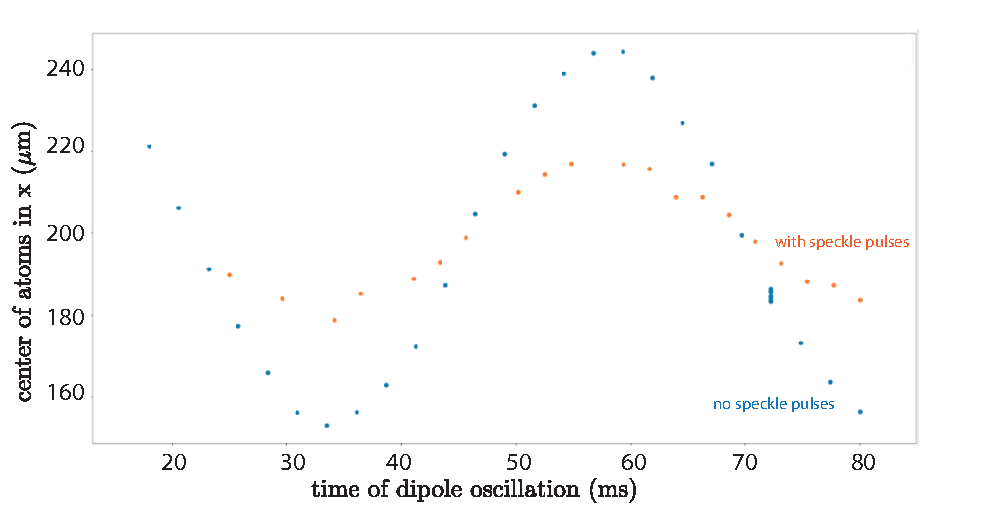
\includegraphics{Chapter6_secs/deceleration_in_dip_osc.pdf}
    \caption{Center-of-mass motion in $x$ direction of atoms during dipole oscillation. The blue dots show a full cycle of dipole oscillation without pulses of the speckle potentials. The orange dots show the dipole oscillation of atoms with the same initial velocity as the blue dots show, but with a $1\ {\rm ms}$ speckle pulse at $21\ {\rm ms}$. The average speckle potential depth is $\approx 640\ {\rm Hz}$.}
    \label{fig:deceleration_in_dip_osc}
\end{figure*}

The amplitude of the oscillation shown by the orange dots is smaller than the amplitude shown by the blue dots. We fit a sinusoidal function to both and infer the velocities of the atoms at $t=21\ {\rm ms}$. Without the pulse of speckle potential at $t=21\ {\rm ms}$, the velocity of the atoms is $v_0$, $mv_0/\hbar = 1.8k_r$. With the pulse, the velocity of the atoms is $v_f$, $mv_f/\hbar = 0.7k_r$. This measurement demonstrated that a speckle potential pulse with an average potential depth of $\approx 640\ {\rm Hz}$, can have a significant deceleration effect on atoms within $1\ {\rm ms}$. This allows us to measure the deceleration of atoms evolving in speckle potentials in our optimized dipole trap, without having to reduce the $x$ trapping frequency.

Using this method, we measured the deceleration of atoms at different velocities $v_0$ after pulses of speckle potential for $1\ {\rm ms}$ with an average potential depth of $\approx 500\ {\rm Hz}$. Fig.~\ref{fig:spinless transport} shows the experimental measurements compared with the numerical simulation results. The red circles in Fig.~\ref{fig:spinless transport} show the experimental results. In the numerical simulations, we make atoms with different initial velocities evolve under speckle potentials with different potential depth for $1\ {\rm ms}$ and measure the final velocities. The initial velocities range from $0.2\frac{\hbar k_r}{m}$ to $2.2\frac{\hbar k_r}{m}$. The blue curve and the yellow curve in Fig.~\ref{fig:spinless transport} correspond to speckle potential depth of $500\ {\rm Hz}$ and $800\ {\rm Hz}$, respectively. In the experiments, the average speckle potential depth is inferred from Fig.~\ref{fig:avg_speckle_poten}. As discussed in Sec.~\ref{long_pulse}, we use the stationary width of the momentum distribution after long-term speckle pulses to measure the average speckle potential. Here the deceleration measurement is done with a PD reading of $1.0\ {\rm V}$, which corresponds to an average speckle potential of $\approx 500\ {\rm Hz}$. For initial velocities $v_0$, the measured final velocities $v_f = \frac{\hbar k_r}{m}$ are lower than the final velocities in the simulation with average speckle potential of $500\ {\rm Hz}$, and are close to those in the simulation with average speckle potential of $800\ {\rm Hz}$. There are a few potential causes that can lead to the gap. First, in the measurements of the stationary width of momentum distribution after long-term pulses of speckle potential shown in Fig.~\ref{fig:avg_speckle_poten}, the stationary width is noisy which leads to uncertainty in the calculation of average speckle potential depth. Second, as discussed in Sec.~\ref{short_pulse_sec}, it is hard to measure the $k_c$ of the optical speckle potentials used in the experiments accurately. The difference in $k_c$ of speckle potentials used in the simulations and the experiments can also lead to this gap.

%we fit a Gaussian function to the spatial distribution of atoms to extract the center-of-mass positions, as the dots in Fig.~\ref{fig:deceleration_in_dip_osc} show. Then we fit a sinusoidal function to the center-of-mass positions of atoms when they oscillate in a dipole trap, and infer the velocity at $t=21~{\rm ms}$. The Gaussian fits and the inference of velocities from the sinusoidal fits also introduce uncertainties.

\begin{figure*}
    \centering
    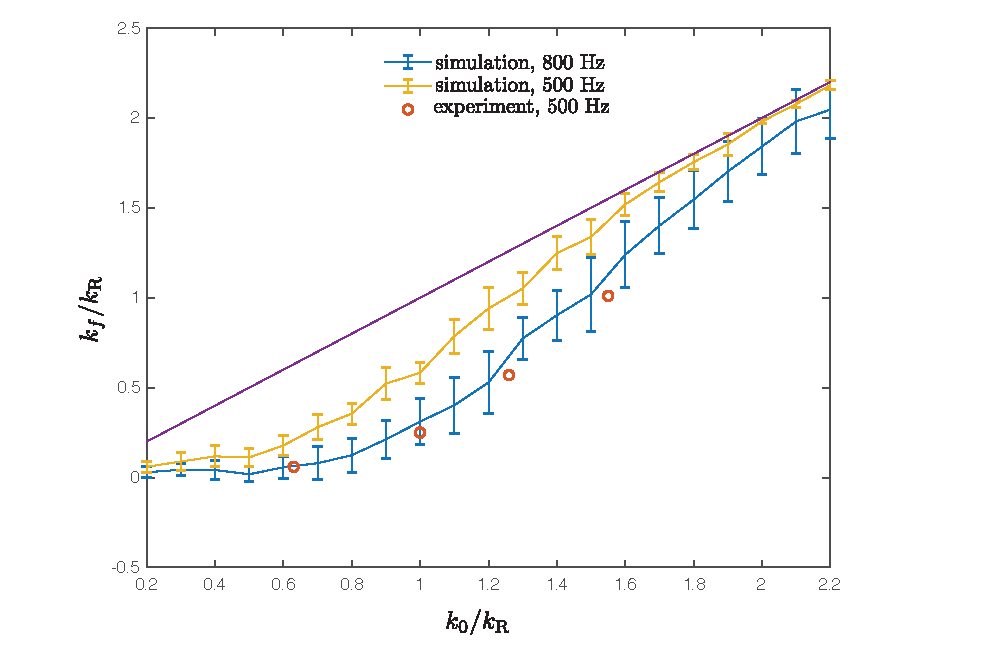
\includegraphics{Chapter6_secs/spinless_transport.pdf}
    \caption{Deceleration of atoms after a $1\ {\rm ms}$ pulse of the speckle potentials. The red circles are the results of measurements in the experiments. The average speckle potential depth inferred from the photo diode reading is $\approx 500\ {\rm Hz}$. The blue curve and the yellow curve are the results of numerical simulations. The blue curve is the final velocities vs the initial velocities after evolving under speckle potentials with average potential depth of $800\ {\rm Hz}$, and the yellow curve is for speckle potential with average potential depth of $500\ {\rm Hz}$. Both the blue curve and the yellow curve are averaged over 20 speckle realizations and the error bars show the standard deviations. The purple line is diagonal. }
    \label{fig:spinless transport}
\end{figure*}